在Cytoscape中有四种创建网络的方法:
\begin{enumerate}
\item 导入预设的格式化网络文件。
\item 导入预设的未格式化的文本文件或Excel文件。
\item 从Web Service导入网络。
\item 创建一个空网络,然后手动地添加节点和边。
\end{enumerate}
\section{导入确定格式的网络文件}

在\ref{ch06}中介绍的所有网络文件格式都可以导入到Cytoscape中。点击File $\rightarrow$ Import $\rightarrow$ Network (multiple file types),在弹出的``Import Network''窗口中就可以把网络文件导入到Cytoscape中。可以是本地计算机上的网络文件,也可以是远程计算机上的(用URL)。

 \subsection{从本地计算机上导入网络}
在缺省情况下,Cytoscape会从本地计算机加载网络。

在Import Networks中会显示缺省的``Data Source Type: Local,'',意思就是从本地计算机导入网络文件。 点击Select按钮选择要加载的网络文件(只有Cytoscape能识别的文件才会显示出来),然后点击Import按钮把网络加载到Cytoscape中。在Cytoscape的sampleData的文件夹中能找到一些不同类型的网络文件。 

SIF、GML和XGMML格式的网络文件也可以在命令行中用-N选项直接导入。

\begin{center}
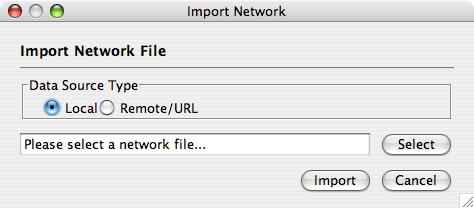
\includegraphics[width=\textwidth]{images/network_import_dialog1_25.png} 
\end{center}

\subsection{从远程计算机上导入网络(URL导入)}
在Import Networks中还可以使用URL导入网络文件。首先把Data Source Type设置成Remote,然后手动填写或是用书签插入合适的URL。点击文本域右边的箭头就能访问收藏的URL。(书签管理器的详细信息参阅Preferences中的Bookmark Manager一节。还可以把浏览器中的URL拖拽到URL文本框中。指定好URL后,点击Import按钮就能加载网络。

\begin{center}
 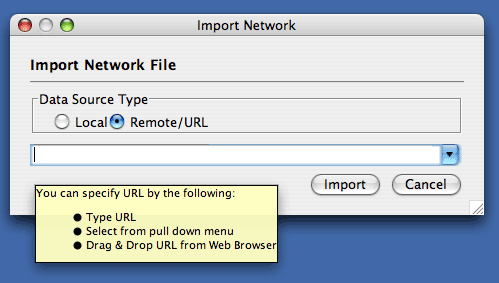
\includegraphics[width=\textwidth]{images/network_import_dialog2_25.png} 
\end{center}

从URL地址导入网络一定要注意一点。由于Cytoscape主要(但不是完全)是根据文件的后缀来判断文件的类型,所以如果URL中的文件的后缀不合适的话,在导入网络时就有可能遇到麻烦。如果Cytoscape没能在URL识别出有意义的文件名和后缀,它就会根据MIME类型来猜测文件的类型。如果所有的导入句柄就无法识别MIME类型,导入就会失败。

在导入网络时有可能遇到的另一个问题就是防火墙,导致无法访问文件。为了解决这个问题,Cytoscape支持使用代理服务器。在 Edit $\rightarrow$ Preferences$\rightarrow$ Proxy Server...中就可以设置代理服务器。在Preference有这方面的更多信息。

\section{导入格式灵活的表格文件}
从2.4版开始,Cytoscape就能通过Edit $\rightarrow$ Import $\rightarrow$ Network from Table (Text/MS Excel)...从文本文件和Excel文件中导入网络。在弹出的窗口中可以设置处理文件的各种选项。还能预览当前设置对文件的处理结果。修改设置时,预览窗口也会自动更新。除了设置文件的处理方法,用户还必须指定Source节点和Target节点,还可以这是边的类型。

\begin{center}
 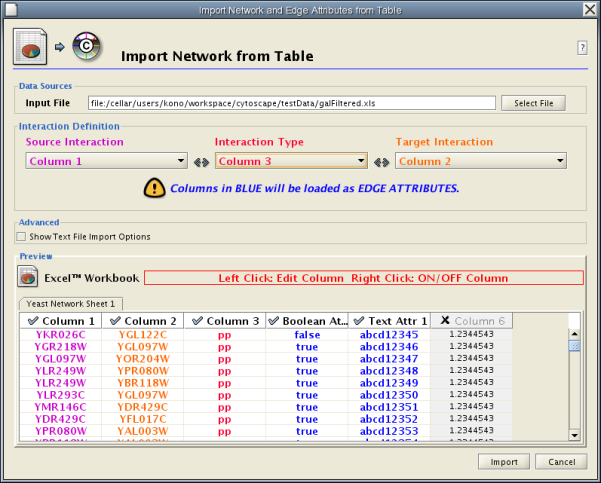
\includegraphics[width=\textwidth]{images/network_table_import.png} 
\end{center}

\subsection{支持的文件类型}
``Import Network from Table''功能支持按特定符号分割的文本文件,和单工作表的微软Excel文件。下面就是一个例子:

\medskip

{\tiny
\begin{tabular}{cccccc}
source  &target&  interaction&  boolean attribute&  string attribute&        floating point attribute\\
YJR022W &YNR053C &pp     & TRUE  &  abcd12371    &   1.2344543\\
YER116C &YDL013W &pp     & TRUE   & abcd12372    &   1.2344543\\
YNL307C &YAL038W &pp     & FALSE  & abcd12373    &   1.2344543\\
YNL216W &YCR012W &pd     & TRUE   & abcd12374    &   1.2344543\\
YNL216W &YGR254W &pd     & TRUE   & abcd12375    &   1.2344543
\end{tabular}}


网络文件至少要有两列:一列是起点,一列是终点。相互作用的类型是可选的。所以,最简单的网络表格应该是这样的:

\begin{verbatim}
YJR022W YNR053C
YER116C YDL013W
YNL307C YAL038W
YNL216W YCR012W
YNL216W YGR254W
\end{verbatim}

在网络文件中,每一行都是一条边以及这条边的属性。所以,网络文件是网络数据和边属性的组合。当然,表中的某些列可能并不是边的属性。遇到这种情况,就可以选择不导入这些列,在预览窗口中点击这一列的表头就是了。例如,在导入下面这种表时,这个功能有很有用:

\begin{verbatim}

Unique ID A  Unique ID B  Alternative ID A
Alternative ID B  Aliases A Aliases B Interaction
detection methods   First author surnames   Pubmed
IDs   species A species B Interactor types  Source
database Interaction ID  Interaction labels
Cross-references  Associated Files  Experiment
files  Experiment labels Different techniques
Different Pubmed articles Different sources Weight

7205 5747 TRIP6   PTK2 Q15654  Q05397-1  vv|HPRD
Currently not available
14688263|15892868(Marcotte)  Mammalia  Homo
sapiens protein|protein HPRD|Marcotte   0 Thyroid
hormone receptor interactor 6-FAK-|PTK2-TRIP6
NA(HPRD)|NA(Marcotte)
HPRD/02859_psimi.xml|other/ORIGINAL_DATA_MARCOTTE.txt
vv(HPRD/02859_psimi.xml)|HPRD(other/ORIGINAL_DATA_MARCOTTE.txt)
17651(ExptRef)|Marcotte 2 2 2 2

4174 7311 MCM5 UBA52   P33992  P62987
neighbouring_reaction   Currently not available
15608231(Reactome)   Homo sapiens Homo sapiens
protein|protein Reactome  1 P33992-P62988
Reaction:68944<->Reaction:68946(Reactome)|Reaction:68946<->
Reaction:68944(Reactome) other/ORIGINAL_DATA_MARCOTTE.txt
neighbouring_reaction(other/REACTOMEhomo_sapiens.interactions.txt)
Reactome 1 1 1 1

7040 7040 TGFB1   TGFB1   P01137  P01137  nmr:
nuclear magnetic resonance Currently not available
8679613 Homo sapiens Homo sapiens protein|protein
BIND 2 TGFB1-TGFB1- 72085(BIND)
BIND/bind_taxid9606.1.psi.xml   nmr: nuclear
magnetic resonance(BIND/bind_taxid9606.1.psi.xml)
NotAvailable 1 1 1 1

\end{verbatim}

 This data file is a tab-delimited text and contains network data (interactions), edge attributes, and node attributes. To import network and edge attributes from this table, you need to choose Unique ID A as source, Unique ID B as target, and Interactor types as interaction type. Then you need to turn off columns used for node attributes (Alternative ID A, species B, etc.). Other columns can be imported as edge attributes. 

 The network import function cannot import node attributes - only edge attributes. To import node attributes from this table, please see the Attributes section of this manual. 

 Note (1): This data is taken from the \emph{A merged human interactome}
 datasets by Andrew Garrow, Yeyejide Adeleye and Guy Warner (Unilever, Safety and Environmental Assurance Center, 12 October 2006). Actual data files are available at \url{http://www.cytoscape.orghttp://cytoscape.org/cgi-bin/moin.cgi/Data}\_Sets/
 
\subsection{Basic Operations}

 To import network text/Excel tables, please follow these steps: 
\begin{enumerate}
\item Select File $\rightarrow$ Import $\rightarrow$ Network from Table (Text/MS Excel)... 
\item Select a table file by clicking on the Select File button. 
\item Define the interaction parameters by specifying which columns of data contain the Source Interaction, Target Interaction, and Interaction Type. Setting the Interaction Type as Default Interaction will result in all interactions being given the value pp; this value can be modified in Advanced Options (below). 
\item (Optional) Define edge attribute columns, if applicable. Network table files can have edge attribute columns in addition to network data.
\begin{itemize}
\item Enable/Disable Attribute Column - By \emph{left}
-clicking on a column header in the preview table, you can enable/disable edge attributes. If the header is checked and entries are blue, the column will be imported as an edge attribute. For example, the table below shows that columns 1 through 3 will be used as network data, column 4 will not be imported, and columns 5 and 6 will be imported as edge attributes. 
\begin{center}
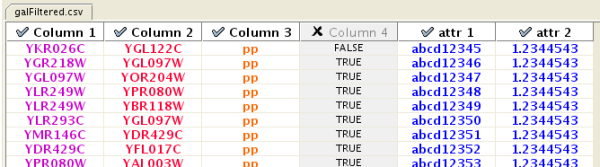
\includegraphics[width=\textwidth]{images/network_table_sample.png} 
\end{center}

\item 

 Change Attribute Name and Data Types - If you \emph{right}
-click on a column header in the preview table, you can modify the attribute name and data type. For more detail, see ``Modify Attribute Name/Type'' below. 

\end{itemize}
\item Click the Import button. 
\end{enumerate}

\subsection{Import List of Nodes Without Edges}
 Table Import feature supports list of nodes without edges. If you select source column only, it creates a network without interactions. This feature is usufl with node expansion function available from some web service clients. Please read the section \emph{Importing Networks from External Database}
 for more detail. 

\subsection{Advanced Options}
\begin{center}
 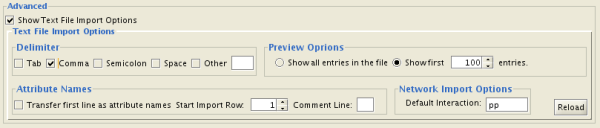
\includegraphics[width=\textwidth]{images/network_import_advanced.png} 
\end{center}

 You can select several options by checking the Show Text File Import Options checkbox. 
\begin{itemize}
\item Delimiter: You can select multiple delimiters for text tables. By default, Tab and Space are selected as delimiters. 
\item Preview Options: When you select a network table file, the first 100 entries will be displayed in the Preview panel. To display more entries, change the value for this option. If you want to show all entries in the file, select ``Show all entries in the file''. You will need to click the Reload button to update the Preview panel. 
\item Attribute Names \begin{itemize}
\item Transfer first line as attribute names: Selecting this option will cause all edge attribute columns to be named according to the first data entry in that column. 
\item Start Import Row: Set which row of the table to begin importing data from. For example, if you want to skip the first 3 rows in the file, set 4 for this option. 
\item Comment Line: Rows starting with this character will not be imported. This option can be used to skip comment lines in text files. 
\end{itemize}
\item Network Import Options: If the Interaction Type is set to Default Interaction, the value here will be used as the interaction type for all edges. 
\end{itemize}
 
\subsection{Modify Attribute Name/Type}

\begin{center}
 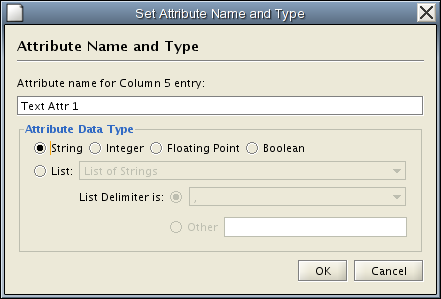
\includegraphics[width=\textwidth]{images/network_table_attr_dialog1.png} 
\end{center}

 Attribute names and data types can be modified here. 
\begin{itemize}
\item Modify Attribute Name - just enter a new attribute name and click OK. 
\item Modify Attribute Data Type - The following attribute data types are supported: \begin{itemize}
\item String 
\item Boolean (True/False) 
\item Integer 
\item Floating Point 
\item List of (one of) String/Boolean/Integer/Floating Point 
\end{itemize}
\end{itemize}
 Cytoscape has a basic data type detection function that automatically suggests the attribute data type of a column according to its entries. This can be overridden by selecting the appropriate data type from the radio buttons provided. For lists, a global delimiter must be specified (i.e., all cells in the table must use the same delimiter). 

\section{Import Networks from Web Services}
 From version 2.6.0, Cytoscape has a new feature called \textbf{Web Service Client Manager}
. Users can access verious kinds of databases through this function. Please read \emph{\textbf{Importing Networks and Attributes from External Database}
}
 for more detail. 

\section{Edit a New Network}
 A new, empty network can also be created and nodes and edges manually added. To create an empty network, go to File $\rightarrow$ New $\rightarrow$ Network $\rightarrow$ Empty Network, and then manually add network components using the Editor in CytoPanel 1 (see the Editor chapter for more details). 
